\section{Naming the principal driver from MMD, HSIC, and R-risk}
\label{sec:kernel-drivers}

Sites in one federation do not share a shift.
A mean shift, a variance change, a linear concept, a sine, a product, and a site whose labels have been replaced by noise can all be present at once.
Stacking the rows and computing one MMD or one R-risk answers a different question.
That overall number cannot name a site, and on the heterogeneous federation below it is the wrong size: the pooled R-risk is \(0.005\), while the noisiest site has raw R-risk \(0.388\).

The call uses three site scores, in a fixed order, on that site's own reference window and its own new window.

\par\noindent\textbf{MMD names the covariate driver.}
It is the unbiased squared RBF discrepancy between the two windows.
The kernel width is the median distance on the pooled windows and is held fixed when a column is removed, so the leave-one-column drop is the share of the discrepancy that column carries.
MMD does not see the label and is not multiplied by outcome skill.

\par\noindent\textbf{R-risk is the concept dose, and skill decides whether it counts.}
For the Gaussian designs the reference regression is ordinary least squares, which is the shared conditional mean.
The R-learner then explains the residual with a treatment effect of the environment indicator.
The effect is the better of a linear tau, a quadratic tau, and a degree-5 polynomial in one coordinate, chosen by cross-fit loss.
The reported R-risk is the fraction of residual variance that effect removes.
A noise site, whose new labels are standard normal, has mean raw R-risk \(0.388\) on the heterogeneous federation.
Its new-window \(R^2\) is \(0\), so the gated score \(R\text{-risk}\times\mathrm{skill}\) is \(0\).
On that federation the ungated R-risk ranks every concept site behind the noise site.
The gated score ranks every concept site ahead of it.

\par\noindent\textbf{HSIC names the coordinate when one column carries the concept.}
The residual is the new label minus the reference regression.
HSIC between that residual and the environment indicator is the scalar dependence.
The coordinate score is the increase, from the reference window to the new window, of HSIC between that column and the residual.
A sine of amplitude one on a column that the baseline regression does not use has a small global R-risk and a coordinate HSIC that peaks on the planted column in every replicate of the unit check.
The concept score kept for the call is the larger of the gated R-risk and that peak times the same skill.
No fourth site score enters the call.

A site is named only when its score beats the median of the lower half of the federation by an absolute gap: \(0.006\) for MMD and \(0.03\) for the concept score.
The principal covariate driver is the leader of the MMD call.
The principal concept driver is the leader of the concept call.
If the gap does not open, that arm names nobody.

\subsection{What was scored}
\label{sec:kernel-designs}

Every synthetic block from the aggregation note is included, with \(d=10\), \(200\) reference rows and \(200\) new rows at each of six sites, and four seeds.
Three sites are shifted and three are clean, except the null block, in which none are shifted.
Covariate shifts redraw the label from the original conditional mean after the covariate move, so a mean shift is not an intercept change in disguise.
Concept shifts keep \(X\) and add a term: linear in \(X_2\), sine in \(X_5\), cubic in \(X_3\), the product \(X_2 X_4\), or a threshold in \(X_4\).
Amplitudes match the note except where a line below says the shift is below the floor.
Two further blocks put unlike shifts in one federation.
The mixed block has two mean-shift sites, two linear concept sites, one site with both a mean shift and a sine, and one clean site.
The heterogeneous federation has ten sites: two clean, a mean shift, a scale change, a mixture, a linear concept, a sine, a product, a mean shift plus a sine, and one noise site.
The ten-site concept generator is also run on Gaussian covariates, with the same four roles as the ACS benchmark and with no planted covariate shift.

\begin{table}[t]
\centering
\caption{Heterogeneous federation.
Mean over four seeds and the sites of each role.
Skill is out-of-fold \(R^2\) on the new window.
The concept score is gated.
The noise site leads raw R-risk and has concept score zero.}
\label{tab:kernel-roles}
\small
\begin{tabular}{lrrrrrr}
\toprule
Role & MMD & HSIC & R-risk & Skill & Gated R-risk & Concept score \\
\midrule
Clean & 0.001 & 0.007 & 0.009 & 0.797 & 0.007 & 0.023 \\
Covariate & 0.047 & 0.009 & 0.011 & 0.845 & 0.009 & 0.026 \\
Concept & 0.001 & 0.028 & 0.069 & 0.796 & 0.059 & 0.157 \\
Mixed & 0.025 & 0.017 & 0.022 & 0.822 & 0.018 & 0.125 \\
Noise & 0.002 & 0.122 & 0.388 & 0.000 & 0.000 & 0.000 \\
\bottomrule
\end{tabular}
\end{table}

Table~\ref{tab:kernel-roles} is the separation the call uses.
Covariate sites lead MMD and sit with the clean sites on the concept score.
Concept sites lead the concept score and sit with the clean sites on MMD.
The mixed site is elevated on both.
The noise site leads raw HSIC and raw R-risk and is removed by the skill factor.
In all four seeds the named covariate driver is the mixture site, and the named concept driver is either the linear site or the sine site.
The noise site is never named.
The product site is the weak concept: its score often stays under \(0.03\), so the called set does not always contain every concept site.
The principal site is still a concept site in every seed.
Site-level coordinate recovery on this federation, counting a hit when the top leave-one-column of the matching arm is one of the planted columns, is \(1\).

\begin{table}[t]
\centering
\caption{Principal-driver hits over four seeds.
A hit is a named site of the right kind, or nobody when that kind of shift is absent.
Precision is the fraction of called sites whose role matches the arm.}
\label{tab:kernel-hits}
\small
\begin{tabular}{llcc}
\toprule
Design & What moves & Covariate hit & Concept hit \\
\midrule
Heterogeneous, 10 sites & unlike shifts and noise & 1.00 & 1.00 \\
Mixed block & two covariate, two concept, one mixed & 1.00 & 1.00 \\
Mean shift \(1.5\) on \(X_0\) & one coordinate & 1.00 & 1.00 \\
Mean shift \(0.5\) on \(X_0\) & one coordinate, smaller & 0.75 & 0.75 \\
Mixture on \(X_0\) & one coordinate & 1.00 & 0.50 \\
Scale \(\times 1.6\) on \(X_0\) & one coordinate, thin & 0.00 & 0.75 \\
Linear concept & \(X_2\) & 1.00 & 1.00 \\
Sine concept & \(X_5\) & 1.00 & 1.00 \\
Cubic concept & \(X_3\) & 1.00 & 1.00 \\
Threshold concept & \(X_4\) & 1.00 & 1.00 \\
Product \(X_2 X_4\) & two coordinates, weak & 1.00 & 0.00 \\
Null & nothing & 1.00 & 0.75 \\
Binary ten-site concept & no covariate shift & 1.00 & 1.00 \\
\bottomrule
\end{tabular}
\end{table}

Table~\ref{tab:kernel-hits} is the full synthetic list.
Where the shift is carried by one coordinate and the dose is not small, the matching arm is right in every seed and the other arm names nobody.
A mean of \(0.5\) is the edge of the MMD floor: one seed does not open the gap.
A scale of \(1.6\) on one of ten coordinates does not.
Concordance of MMD for that scale, shifted against clean, is \(0.611\).
The unit product does not open the concept gap either.
Its leave-one-column HSIC still lands on a planted coordinate in \(0.833\) of site replicates, which is a coordinate fact and not a site call.
The mixture block names the covariate driver in every seed and a spurious concept driver in two seeds.
The null block names a spurious concept driver in one seed.
Those three rows are the false-call rate of the \(0.03\) floor.

On the binary ten-site generator, MMD concordance of concept sites against clean sites is \(0.412\).
The concept score concordance is \(0.912\) against clean sites and \(1\) against the noise site.
Ungated R-risk against the noise site is \(0.800\).
The named concept driver is a concept site in every seed, and no covariate driver is named.
The called concept set is the strong nonlinear sites rather than all five structured sites: recall is \(0.400\), precision is \(1\).

\subsection{The pooled number and the column that carries the shift}
\label{sec:kernel-pool}

\begin{table}[t]
\centering
\caption{Pooled score against the strongest site.
Means over four seeds.
On the heterogeneous federation the largest raw R-risk is the noise site.
The largest gated R-risk is a concept site.
The pool sits near zero in both columns.}
\label{tab:kernel-pool}
\small
\begin{tabular}{lrrrr}
\toprule
Design & Pooled MMD & Max MMD & Pooled R-risk & Max R-risk \\
\midrule
Heterogeneous & 0.003 & 0.075 & 0.005 & 0.388 \\
Mixed block & 0.013 & 0.075 & 0.022 & 0.191 \\
Mean shift \(1.5\) & 0.013 & 0.078 & 0.002 & 0.014 \\
Binary ten-site & 0.000 & 0.002 & 0.007 & 0.203 \\
\bottomrule
\end{tabular}
\end{table}

Table~\ref{tab:kernel-pool} is why the site scores are computed before the stack.
Three of six sites carry a mean shift of \(1.5\), and the pooled MMD is already a sixth of the strongest site.
One noise site in ten makes the pooled R-risk \(0.005\) while that site's own raw R-risk averages \(0.388\).
Gating has to happen at the site.
A gate applied to the pooled residual has nothing left to multiply: the concept sites have been averaged with clean sites and with noise.

\begin{figure}[t]
\centering
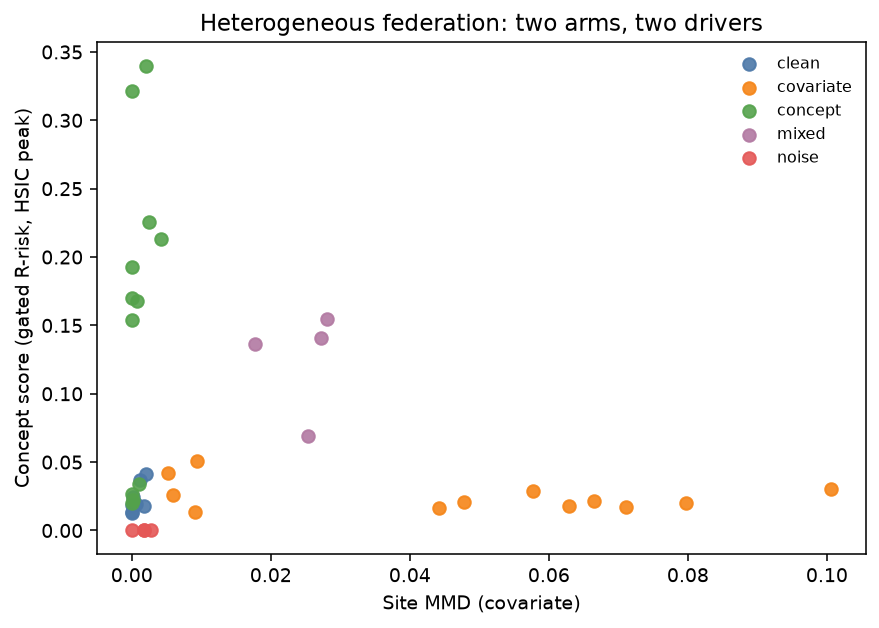
\includegraphics[width=0.86\textwidth]{../results/figures/kernel_driver_scatter.png}
\caption{Heterogeneous federation, four seeds.
Covariate sites sit to the right.
Concept sites sit up.
The noise site is at the origin because its concept score is gated to zero.
The mixed site is the only role that moves on both axes.}
\label{fig:kernel-scatter}
\end{figure}

When every shifted site plants the same column, the pooled leave-one-column vector recovers it.
A mean shift of \(1.5\) on \(X_0\) has MMD-weighted and pooled coordinate AUC both equal to \(1\).
A linear concept on \(X_2\) has pooled R-risk coordinate AUC \(1\).
The heterogeneous federation is the case the pool does not cover.
Sites plant different columns, and the noise site uploads a large raw residual.
The pooled R-risk coordinate vector has AUC \(0.365\) against the planted concept columns and its top column is in the support in \(0.25\) of seeds.
The same vector, averaged with weights proportional to gated R-risk, has AUC \(0.771\) and its top column is in the support in every seed.
The HSIC vector with those weights has AUC \(0.792\) and the same perfect top-column rate.
On the binary generator the HSIC vector weighted by gated R-risk has AUC \(0.983\) and precision \(0.917\); the pooled HSIC vector has AUC \(0.725\) and precision \(0.583\).

The order is the identification.
MMD, ungated, names the covariate driver and the column that carries it.
R-risk names the concept dose.
Skill multiplies R-risk and the HSIC peak, which is what removes the noise site after aggregation would already have mixed it in.
The weighted leave-one-column vector is then the principal coordinate.
The pooled statistic is the check that this weighting was doing something the stack does not do by itself.
